% No new page; first page call under this section. see ProjectStructureSrc . 
\visHeader

Now that everything is installed and setup properly, let's take a closer look at the different workspaces and our workflow.
Before we continue, please make a few slight adjustments to EA so you can easily compare your current workspace to our screenshots:
\begin{itemize}

\item[$\blacktriangleright$] Select ``Tools/Options/Standard Colors'' in EA, and set your colours to reflect Fig.~\ref{fig_standardColoursEA}.
This is advisable but you're of course free to choose your own colour schema.

\begin{figure}[htbp]
  \centering
  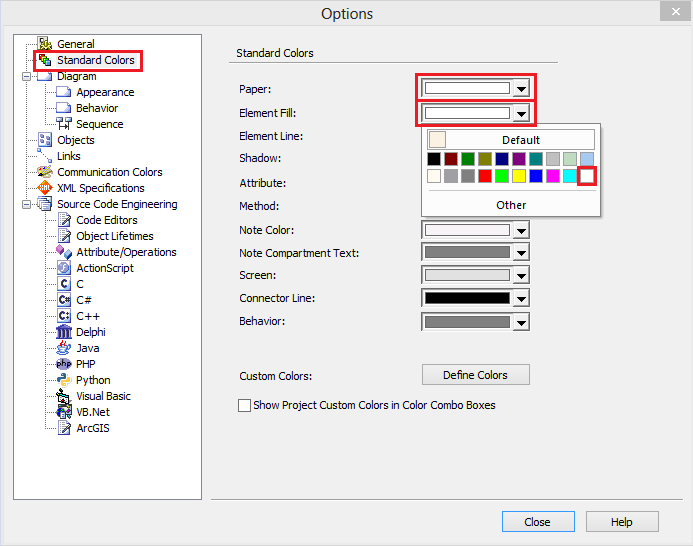
\includegraphics[width=0.8\textwidth]{standardColours}
  \caption{Our choice of standard colours for diagrams in EA.}
  \label{fig_standardColoursEA}
\end{figure}

\item[$\blacktriangleright$] In the same dialogue, select ``Diagram/Appearance'' and reflect the settings in Fig.~\ref{fig_standardAppearanceEA}.
Again, this is just a suggestion and not mandatory.

\item[$\blacktriangleright$] Last but not least, and still in the same dialogue, select ``Source Code Engineering'' and be sure to choose ``Ecore'' as the default language for code generation (Fig.~\ref{fig_standardSCEEA}). This setting is very important.
\end{itemize}

In your EA ``workspace'', actually referred to as an \emph{EA project}\footnote{Words are set in italics when they represent concepts that are introduced or defined  in the corresponding paragraph for the first time.}, take a careful  look at the project structure:  The root node \texttt{Demo}\footnote{Words set  in a \texttt{mono-space font} refer to things that you should find in a tool,  dialogue, figure or code.} is called a \emph{model}